\section{Manual de usuario}

\subsection{Configuración hardware}

El cartel posee elementos de hardware configurables, los mismos se detallan a continuación:

\begin{table}[ht!]
	\centering
	\caption{Detalle de cada componente configurable.}
	\label{my-label}
	\begin{tabular}{lcp{.65\textwidth}}
		\multicolumn{1}{c}{Elemento}	& Identificación & \multicolumn{1}{c}{Descrición} \\ \hline
		Switch de Power         		& 1              & Encender o apaga el cartel, el cartel no recibe energía eléctrica si esta apagado. \\ \hline
		Switch de Formateo      		& 2              & Formatea la memoria interna, y se carga los datos de fabrica, para este propósito es necesario que se mantenga en ese estado por al menos 3 segundos. \\ \hline
		Jumpers de capacidad 			& 3              & En total son tres. Antes de encender de debe seleccionar la cantidad de módulos esclavos que serán utilizados. \\ \hline
	\end{tabular}
\end{table}

En la figura es posible observar los elementos anteriormente mencionados identificados por su número correspondiente.
% TODO: Sacar fotol esta dado 

\subsubsection{Escalabilidad}
La escalabilidad, es decir, el tamaño del cartel lo determina la cantidad de módulos esclavos conectados entre sí. Este valor se establece activando los jumpers en una configuración determinada. La figura \ref{fig:manual-jumpers} explica como deben establecerse para este propósito.

\begin{figure}[ht!]
	\centering
	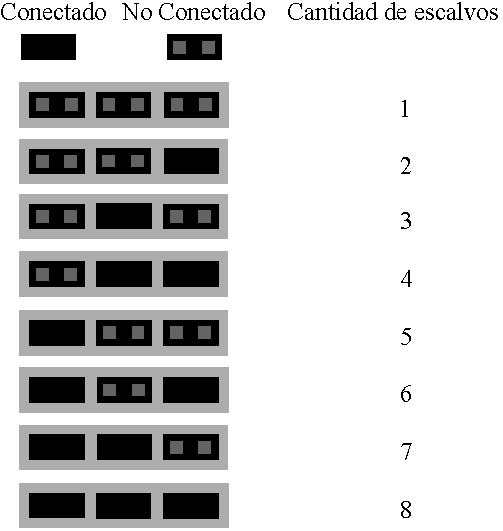
\includegraphics[width=0.6\linewidth]{imagenes/manual/jumper.pdf}
	\caption{Configuración de los jumpers para cada cantidad esclavos conectados.}
	\label{fig:manual-jumpers}
\end{figure}

\subsection{Configuración software}
Del lado del software, al ingresar al panel existe una opción que esta en la parte superior izquierda en la que es posible cambiar la contraseña de acceso y la IP.
